\title{System Dynamics:  Exercise 2 - Predator Prey}
\author{Ryan Spangler}
\date{\today}

\documentclass[12pt]{article}

\usepackage{graphicx}

\begin{document}
\maketitle

\section{Approach}

In this exercise I chose to model a predator-prey system that also incorporates a forage for the prey.  In this way it is a three-tiered system, with predators preying on prey, who forage on forage.  The predators die naturally, or from starvation when no prey is present, but are not directly preyed upon by anything, and therefore their death rate is simpler than that of the prey or the forage, which is inversely proportional to the population of consumers a level above in the food chain.  Likewise, the forage consumes ``sunlight'', which in this model is an exogenous factor which directly scales the forage growth rate.  So the birth rate of the forage depends only on the amount of forage present, and is not impacted by the population of any consumable stock, as is the case for the predators and the prey.  

I was interested most in what the interactions between the various populations would be, especially between the predators and the forage, who are only indirectly related through the dynamics of the prey population.  The prey population in this way acts as a kind of mediator between the predators and the forage, and is the only population who is impacted by a large consumer population and also dependent on a consumee population.  I was curious about what effect this would have on the dynamics of the prey population, as it had the potential to undergo both boom periods when the predators were few and the forage plenty, and also bust periods when the predators were everywhere and forage scarce.  I predicted that neither of these extremes would happen often, as if the predators were heavy then the prey would be few and the forage was not likely to be ravaged, and if the forage was high the prey population would be high and the predators would be plentiful.  What I was interested in finding out was how the delays between the size of the various populations would influence the synthesis of conditions between them, and discover the structure behind the oscillating dynamics that characterize predator-prey systems in nature.  

\section{Process}

In this exercise I took a symmetrical approach to the various stocks.  I wanted each stock to stand on its own as a plausible biological population, meaning that each would influence its own birth and death rates, and would show the characteristic exponential dynamics in the absence of any other limiting factors.  These limiting factors came in some form or another for each stock.  For the predators, their death rate is inversely proportional to the size of the prey population.  This way, in the absence of prey the predator population would decline rapidly.  This is in addition to the birth rate of the predator population depending on the size of the prey population.  In this way the prey population influences both the birth and the death rate of the predators, providing reinforcement to the notion that the two populations are linked.  I began the model having a simpler approach, with the size of the prey population affecting only the birth rate of the predators (as they ate more, more predators were conceived), but found this inadequate to achieve the necessary dynamics.  In all of the populations, the consumable population on which it rested had to be tied into both the birth AND the death rates to resemble the RBP I started out with (that of the populations oscillating out of phase with one another, as the effects of the decline or increase in any one of the populations propagate through the system).  

In the following diagram there are three stocks, each with a birth and a death rate, and six parameters, one for each birth and death rate.  There are feedback loops between each population and its various flows: reinforcing for the birth rates and balancing for the death rates.  In addition to those loops, there is a balancing loop between the size of the prey population and the size of the predator population, with an increasing prey population increasing the predator birth rate, which increases the prey death rate, leading to a lower prey population.  There is a symmetrical loop for the prey and the forage, with the prey population reducing the forage which reduces the prey, which leads to an increase in the forage etc.  It is these loops that are behind the oscillating dynamics characteristic of this and other predator-prey systems.  The feedback loops alternatively reinforce and negate the benefits of a larger population, leading to oscillations in all of the populations in a dependent, interlinked way.  

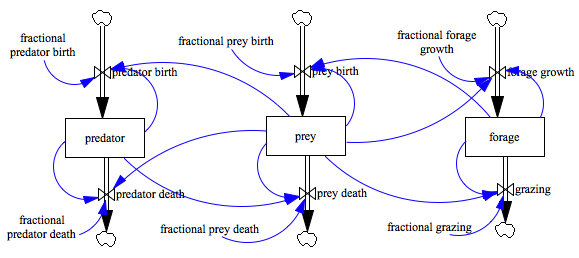
\includegraphics[scale=0.63]{exercise2model.png}

One of the things that became more clear to me with this exercise was the distinction between varying parameters and adding new arrows between stocks or flows.  While I spent a lot of time calibrating the model with various values, it was rare that the actual {\em dynamics} would change through any of this tinkering.  It was only through adding or removing arrows, or dependencies between various elements of the model, that I would get any kind of change in what the model really did.  The times when the dynamics of the model would change through adjusting a parameter it appeared as a kind of ``threshhold'' effect, where the shape of the curve would shift and shift until a certain point was reached where everything would fall to one extreme or another.  Sometimes it would spiral off into infinity, or rapidly decline to zero.  In all cases, if all of the parameters rested within the bounds of these threshholds, the system would have a characteristic dynamic that was invariant inside of these threshholds.  For this reason several times during the course of the exercise I would have spent a good deal of time calibrating the model in its current state, and then discover I wanted to add an arrow somewhere.  This would throw off all of the calibrations and send the system careening off to some extreme, whereupon the calibration process would start all over again.  I found this frustrating at times, and found myself longing for some means to automatically offset parameter values with the new implications of the additional dependency, though I realize this could just be the nature of the beast.  

Also through the calibration process I discovered an interesting thing about this model, which is that it basically only works if the population of consumable is at least an order of magnitude larger than the population of consumer.  Because of this the predators ended up having an initial starting size of 100, the prey 1000 and the forage 10000.  I thought this was an interesting consequence of the structure of a predator prey relationship.   

One concern I had was that when the various threshholds were reached, the model would spiral out of control rather quickly.  There seemed to be a rather narrow band within which the system would function reliably, and a vast area outside of that that would either die quickly or become practically infinite in a short period of time.  One of the aims I developed over the course of this exercise was to discover what makes a model frail and what makes a model robust, and to develop models that have greater tolerances for error and the ability to perform well under a variety of conditions.  From my experience with developing the models I have this is obviously a spectrum, but one that I endeavor to understand more about in the future.

\section{Results}

For the most part, the model exhibited oscillating results, though much more drastic than I expected.  In the times of decline, both predator and prey populations would be close to zero, and when the prey population started rising again in the presence of renewed forage, the predator population would track closely behind, leaving the time of plenty somewhat short-lived:

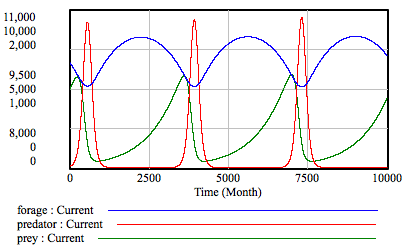
\includegraphics[scale=0.8]{modelbehavior.png}

It seems the combination of both a decreased forage supply and the simultaneous increase of predators led to a swift decline in the prey population.  Of the three, the prey population resembled most closely an exponential increase followed by steep decline.  The predator and the forage population had a similar contour for both increase and decrease, leading to a more smoothly oscillating behavior.  It is also notable that the predator and forage populations were almost perfectly inverse of one another, both being affected at the same time by increasing size of the prey population.  In this way the prey population dominated the results by affecting both the forage and the predators at once, while the other were only indirectly connected through the prey.  

This was in contrast to my initial predictions, where I postulated that the occurrence of both extremes for the prey population, that of both high predation and low forage or vice versa, would not occur very often.  We see here that in fact when the predators are plenty, the forage is not and vice versa.  This also answers my question as to how the two populations who were indirectly connected to one another would interact, and it turns out they tracked each other precisely, if inversely.  The predator and the forage were each a consequence of the prey, and did exhibit any behavior independently of this.  

At times, when the one of the parameters was beyond threshhold I would get results like this:

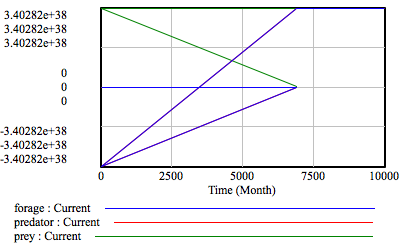
\includegraphics[scale=0.8]{incoherentresults.png}

I cannot explain this graph.  It appears to be linear, with the prey starting at a preposterous value of 3.40282e+38 and declining perfectly to zero sometime before month 7500.  A line for the predator is literally nowhere to be found, and the line describing the prey is forked, going off at two different starting points, in three different linear directions!  I can only assume the values were too extreme for Vensim, but I discovered this behavior alarmingly often, sometimes when tweaking the parameters only by a minimal amount.  This led to a certain degree of doubt in all of the results I was getting from Vensim, as the graph was literally impossible to interpret (with one line having three different values at the same time step!)  Along with other bugs and glitches, my current opinion of Vensim is quite low.  I learned to save often to avoid losing my progress when the inevitable spinning crash would consume all of my cpu and the process would have to be manually killed.  I have seriously been considering looking into Stella(!) as I enjoy the modeling process, but the use of Vensim somewhat tarnishes the experience for me.  

Between the archetypical model behavior and the incomprehensible results I found some other interesting behaviors.  When prey death rate was too low I found a consistent decrease in the ability for the forage population to restore itself.  This led to decreasing dynamics throughout the system:

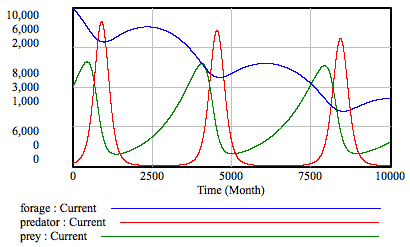
\includegraphics[scale=0.8]{decliningforage.png}

On the flip side of this, there were times when the forage would not be deplenished enough by the prey cycle to overcome its rate of growth, and the entire system would continue oscillating at a higher and more violent rate:

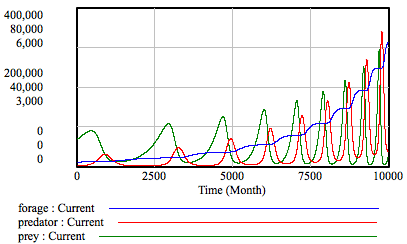
\includegraphics[scale=0.8]{exponentialoscillation.png}

Though the system is oscillating, the amplitudes as a whole are increasing exponentially, which lead to a neverending increase in the activity of the system.  Between these two extremes the system finds a balance between the consumption of the prey and the growth of the forage and the size of the predator population.  The sensitivity I discovered of the system to the various ranges of parameter values is striking.  


\section{Equations}

Here are the resulting equations for the three population stocks, their birth and death rates and the parameters governing them:

\begin{verbatim}
  initial forage population = 10000
  fractional forage growth rate = 0.1
  fractional forage consumption rate = 1e-6
  forage growth rate = fractional forage growth rate * 
    forage population / prey population
  forage consumption rate = fractional forage consumption rate * 
    forage population * prey population
  forage population = INTEGRAL(forage growth rate - 
    forage consumption rate)

  initial prey population = 1000
  fractional prey birth rate = 1e-7
  fractional prey death rate = 1e-5
  prey birth rate = fractional prey birth rate *
    prey population * forage population
  prey death rate = fractional prey death rate * 
    prey population * predator population
  prey population = INTEGRAL(prey birth rate - prey death rate)

  initial predator population = 100
  fractional predator birth rate = 1e-5
  fractional predator death rate = 0.1
  predator birth rate = fractional predator birth rate * 
    predator population * prey population
  predator death rate = fractional predator death rate *
    predator population / prey population
  predator population = INTEGRAL(predator birth rate -
    predator death rate)
\end{verbatim}



\end{document}